\documentclass[11pt,a4paper]{article}
\usepackage[margin=2.2cm]{geometry}
\usepackage{amsmath,amssymb}
\usepackage{booktabs}
\usepackage{enumitem}
\usepackage[dvipsnames]{xcolor}
\usepackage{graphicx}
\usepackage{tcolorbox}
\usepackage[colorlinks=true,linkcolor=NavyBlue,urlcolor=NavyBlue]{hyperref}
\usepackage{microtype}
\setlength{\parskip}{4pt}
\setlength{\parindent}{0pt}
\newcommand{\kT}{k_{\mathrm B}T}
\newcommand{\avg}[1]{\left\langle #1 \right\rangle}
\newcommand{\dd}{\mathrm{d}}
\newcommand{\ie}{i.e.\ }
\newtcolorbox{run}[1][What we run]{colback=Apricot!12,colframe=BurntOrange!70!black,title={#1},fonttitle=\bfseries,left=4pt,right=4pt,top=3pt,bottom=3pt}
\newtcolorbox{pass}[1][Pass criterion]{colback=OliveGreen!8,colframe=OliveGreen!70!black,title={#1},fonttitle=\bfseries,left=4pt,right=4pt,top=3pt,bottom=3pt}
\newtcolorbox{why}[1][Why this step exists]{colback=NavyBlue!6,colframe=NavyBlue!60!black,title={#1},fonttitle=\bfseries,left=4pt,right=4pt,top=3pt,bottom=3pt}
% ##CHRIS 2026-09-17: a fourth box, filled in as each level is actually measured. Numbers come from
% hspist3/validation/paper2_level0_level1_20260916.py and the report 260917_paper2_level0_level1_REPORT.md.
\newtcolorbox{res}[1][What we measured (2026-09-17)]{colback=Plum!8,colframe=Plum!70!black,title={#1},fonttitle=\bfseries,left=4pt,right=4pt,top=3pt,bottom=3pt}
% ##CHRIS 2026-09-18: a fifth box. Every measured result now carries the command that produced it,
% so any level can be re-run without reading a script. Verbatim is allowed inside a tcolorbox body.
\usepackage{fancyvrb}
\newtcolorbox{howto}[1][How to run it yourself]{colback=black!4,colframe=black!55,title={#1},fonttitle=\bfseries,left=4pt,right=4pt,top=3pt,bottom=3pt,fontupper=\small}
\newcommand{\cmd}[1]{\texttt{\footnotesize #1}}

\title{Paper 2, step by step:\\ how we prove the energy-transfer box before we use it}
\author{Cowork note for Chris --- HardDisks / hspist3}
\date{2026-09-16}

\begin{document}
\maketitle

\section*{How to read this}
Paper 1 taught us one rule the hard way: \emph{define the estimator and the pass criterion before looking at whether the number agrees with theory}. Every level below therefore has three boxes --- what we run, what number we compute and against which formula, and what counts as a pass. A level is closed when its pass box is satisfied and the failures are reported with counts, exactly as the health contract does. Nothing from a higher level is trusted before the level below it is closed.

Units as always: $\kT = m = \sigma = 1$, $\sigma = 2r$ the disk diameter, box width $2L_0$, height $H$, $N_s$ disks per compartment, $Z(\eta) = PA/(N\kT)$ from Kolafa--Rottner (KR). Paper~1 gives us two things we now use as instruments: the equation of state $Z(\eta)$ validated for $\eta \le 0.6$, and the sound speed $c_s(\eta)$, which sets the time scale $\tau_{\mathrm{sound}} = L_0/c_s$ of every compartment.

\emph{How good those instruments are (2026-09-17).} $Z$: 171 health-clean pressure trajectories over 45 $(\eta,N)$ cells, two independent estimators (collisional virial and wall momentum flux), agreeing with KR to $+0.15\,\%$ at $\eta = 0.10$ with no size dependence between $N = 400$ and $1600$. $c_s$: A1 v2 gives 7875 trajectories over 35 densities at $N = 100$, and the A2 size ladder ($N = 100$--$2500$, now including $\eta = 0.02$ and $0.05$) extrapolates to KR within about $1\,\%$ at every density up to $\eta = 0.60$; at $N = 100$ the measured $c_s$ sits $1$--$3\,\%$ high, and that offset closes as the box grows. Paper 2 uses $c_s$ only to set scales --- $\tau_{\mathrm{sound}} = L_0/c_s$ and the ratio $u/c_s$ that separates the slow and fast regimes --- so $1\,\%$ is far below anything it can affect: the crossover of Level~2 sits at $u/c_s \approx 0.3$ and its two limits differ by factors, not per cent. \emph{No level of Paper~2 is limited by the precision of the Paper-1 instruments.}

\section{The geometries (the same four as in the hand-calculation note)}

\begin{center}
\small
\begin{tabular}{@{}lp{6.0cm}p{2.5cm}p{5.0cm}@{}}
\toprule
 & Geometry (left $\to$ right) & Energy stores & Closes which level \\
\midrule
A & wall $|$ gas $|$ \textbf{held} divider at $L_0$ ($M = 10^9$) $|$ gas $|$ piston & gas (right; left inert) & 0, 1, 2 \\
C & wall \textbf{--spring--} free wall at $L_0$ $|$ gas $|$ piston & gas, wall, spring & 3 \\
B & wall $|$ empty $|$ held wall $|$ gas $|$ \textbf{free} divider $|$ gas $|$ piston & gas 1, divider, gas 2 & 4 \\
D & wall --spring-- free wall $|$ gas $|$ free divider(s) $|$ gas $|$ piston & all & 5 \\
\bottomrule
\end{tabular}
\end{center}

\textbf{Correction, 2026-09-19.} Geometry A as \emph{run} in Levels 0--2 has gas on \emph{both} sides
of the divider (\cmd{--particles-boxes=50,50}), not a vacuum on the left. It changes nothing, because
the divider is held at $M = 10^9$ and never moves, so the left gas is inert and its compartment does
no work --- but the table said otherwise and the runs are what they are. Geometry~B needs both gases
by construction. Only \textbf{C and D have an empty compartment}, the one behind the spring wall:
gas on that side would push the spring wall from both faces and move the equilibrium the analysis
assumes. The binary now refuses to start in that case (\cmd{--spring-wall} with a non-empty
compartment behind it aborts), and \cmd{--spring-k} is inert unless \cmd{--spring-wall} declares
which wall carries the spring.

\begin{center}
\end{center}
The right piston is prescribed (infinite mass, velocity protocol $u(t)$); it is the only place work enters. Every run uses \texttt{--edmd-acc=0}, drift-first seeding, the strict health contract, and the per-event piston log and per-sample $KE_{L},KE_{R}$ columns that already exist.

% ##CHRIS 2026-09-19: one script that exercises the whole ladder, so the apparatus can be tested
% without reading eight campaign scripts. Steps 1-6 and 8 were run and passed on 2026-09-19.
\section{Running the whole ladder yourself, one step at a time}\label{sec:runall}

Everything below can be exercised from a single script. It runs the same commands as the campaign
scripts with a small seed count, so each step finishes in seconds to a couple of minutes, and it
prints a \textbf{PASS} or \textbf{FAIL} line per step against a stated numeric criterion --- not
something to judge by eye.

\begin{howto}[The command]
\begin{Verbatim}[fontsize=\footnotesize]
cd hspist3/experiments_energy_transfer/_run_scripts
./paper2_run_all.sh                 # list the steps and stop
./paper2_run_all.sh 3               # run step 3 only
./paper2_run_all.sh all             # every step, pausing before each one
./paper2_run_all.sh all --yes       # every step, no pauses
SEEDS=25 JOBS=10 ./paper2_run_all.sh all     # heavier, closer to the campaign
OUT=/tmp/p2 ./paper2_run_all.sh all          # write somewhere else
\end{Verbatim}
\end{howto}

\begin{center}\small
\begin{tabular}{@{}clp{8.4cm}@{}}
\toprule
 & Step & What it proves \\
\midrule
1 & the binary and the box     & the binary exists, is the scientific backend (\cmd{--edmd-acc=0}), and the master box starts clean \\
2 & geometries A B C D         & one seed in each; catches a wall off the $1/24\,\sigma$ grid or gas in the spring compartment \\
3 & Level 0 --- the ledger     & $|W - \Delta KE_{\mathrm{gas}}|/W \le 10^{-4}$ \\
4 & Level 1 --- quasi-static   & $\avg W$ extrapolated to $u \to 0$ against $W_{\mathrm{qs}} = 7.4685 \pm 0.0131\,\kT$, within $2\sigma$ \\
5 & Level 2 --- finite rate    & $\avg W - W_{\mathrm{qs}} = A u^2$ fitted over five speeds, against $A_{\mathrm{step}} = 25.9 \pm 4.3$ \\
6 & Level 3 --- the spring     & geometry C is driven and the trace carries \cmd{SpringE} \\
7 & the pictures               & \cmd{paper2\_geometry\_pictures.sh}: eight PNGs, two render modes per geometry. Needs a screen \\
8 & the analysis scripts       & re-runs the three published analyses; reads only \\
\bottomrule
\end{tabular}
\end{center}

A step FAILs if the binary aborted, if \emph{any} health event fired
(\cmd{forced\_advance}, \cmd{clamp\_repair}, \cmd{overlap\_repair}, \cmd{wall\_overdue}), if fewer
trajectories were produced than asked for, or if its own criterion is missed. The script continues
after a failure so you see the whole picture rather than the first thing that broke.

\emph{Two things to expect.} At a handful of seeds the per-speed $A$ values in step 5 scatter hard
and some come out negative --- that is the thermal spread of $W$ at six seeds, not a defect; only
the fitted $A$ over all five speeds is the check. And until the spring-hygiene build is promoted,
the script prints a note that it is falling back to \cmd{00ALLINONE\_sp}, because
\cmd{--spring-wall} does not exist in the installed binary yet and geometries C and D need it.

\section{Three flags that do not mean what they look like}

Worth reading before running any command below; all three were found the hard way on 2026-09-18 and each moved a
published number.

\begin{howto}[Geometry conventions, measured not assumed]
\textbf{\cmd{--wall-positions} sets the divider CENTRE, and the divider is 1\,$\sigma$ thick}
(\cmd{wall\_thickness\_sigma} in every \cmd{summary.csv}). With the divider at 39.25 the gas-side face is at
\textbf{39.75}, so the right compartment is $78.50 - 39.75 = 38.75\,\sigma$, not the nominal $L_0 = 39.25$. The stop
snapshots confirm it: over 60 runs the closest disk centre to the divider is 40.2867, and a disk of radius 0.5 cannot
approach a face at 39.75 more closely than 40.25.

\textbf{\cmd{--max-right-piston-travel} is measured from the box wall, not from the piston.} The target is
$78.50 - 3.93 = 74.57$, which is where the piston stops; the piston parks at 78.75, so it displaces
$4.18\,\sigma$ while the gas is compressed by exactly the flag value, $3.93\,\sigma$. Use 3.93 in anything about the
gas and 4.18 in anything about the piston.

\textbf{\cmd{--l0} is not the compartment length} --- the binary prints \cmd{L\_eff = L0 - 1}, which is Paper~1's
sound-mode length $L_0 - 2r$, a different quantity again. Always take the compartment from the piston and divider
positions in the trace, as \cmd{paper2\_geometry\_fix\_20260918.py} does.
\end{howto}

\section{Watching one run: the SDL window}

Every number in this note comes from headless runs, because that is the only way 1000 trajectories fit in a lunch
break. But the same binary opens a window, and it is worth looking at once --- for a figure, for a talk, or to check
that the geometry is what you think it is.

\textbf{Corrected 2026-09-19.} The earlier version of this section said ``drop \cmd{--headless}''. That is wrong and it
is why the window seemed to flash and vanish: \cmd{--experiment=energy\_transfer} is a self-contained driver that
\emph{never renders}, with or without \cmd{--headless}. The window belongs to the interactive loop, which you reach
with \cmd{--show-simulation}. And because every stage used to fire automatically, there was nothing to see even when a
window did open. Both are fixed by \cmd{--demo}: the run starts paused with the divider held and the piston parked, each
stage begins on a key, and a HUD line says what the box is doing. \cmd{--demo} is GUI-only --- headless output is
byte-identical with and without it (3-seed gate on traces and event logs).

\begin{howto}[Geometry A --- the Level 1/2 box, one divider (verified 2026-09-19)]
\begin{Verbatim}[fontsize=\scriptsize,frame=single,samepage=true]
cd hspist3
./00ALLINONE --show-simulation --demo --mode=edmd --edmd-acc=0 \
  --seed-drift-order=drift-first --particles=100 --particles-boxes=50,50 \
  --particle-radius=0.5 --l0=39.25 --height=10 --num-walls=1 --wall-positions=39.25 \
  --wall-mass-factors=1000000000 --wall-thickness=0.05 \
  --piston-right-protocol-mode=step --velocity-right-piston-step=0.02 \
  --max-right-piston-travel=3.93 --wall-hold-steps=2000 --steps=40000 \
  --fixed-dt=0.4 --energy-measurement --eff-output=wall-ke --kbt1 --seed=9200
\end{Verbatim}
\textbf{What you will see.} A window opens \emph{paused}, 50 disks either side of an immovable divider, the piston
parked at the right wall, and a HUD reading \cmd{HOLD | t=0.0 | piston x=78.75 | divider x=39.25}. Press \cmd{SPACE}
to run, \cmd{R} to release the divider, then \cmd{P} to start the piston; the HUD switches to
\cmd{PISTON step u=0.020} and $W_{\mathrm{in}}$ starts climbing. At $u = 0.02$ the push is $200\,\sigma$-time,
about 12\,000 steps --- roughly two minutes at the default pace, which is what you want to talk over; \cmd{+} and
\cmd{-} double and halve it live (render pacing only, $\dd t$ is never touched).

\begin{center}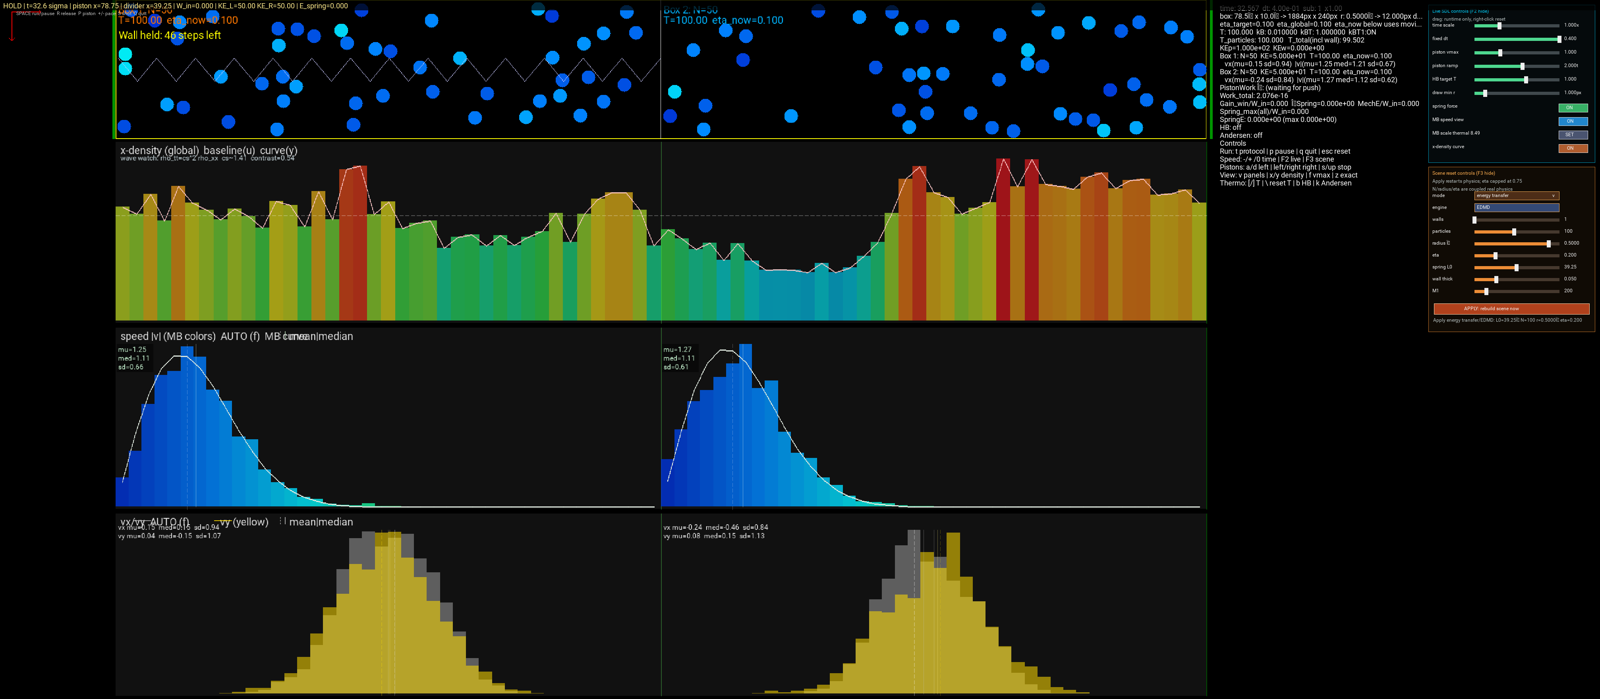
\includegraphics[width=\linewidth]{../paper2_energytransfer/experiments/final/260919_demo_geomA.png}\end{center}

Swap \cmd{--piston-right-protocol-mode=ramp --piston-ramp-time=40} to watch the gentle launch beside the step, which
is Level~2's item~1 in one picture; raise $u$ to 3--10 for the single-hit regime of Section~\ref{sec:fast}.

\textbf{Do not take data this way.} Window runs are for looking; every campaign number in this note is headless,
\cmd{--edmd-acc=0}, with the health contract enforced.
\end{howto}

Geometry~A is what Levels 0--2 measure, but the paper's first figure will be geometry~D: piston, gas, a heavy free
divider, a second gas, and a spring-loaded wall. That runs today, and watching it is the quickest way to see why the
later levels are worth doing.

\begin{howto}[Geometry D --- two walls and a spring, Paper 2's figure 1 (verified 2026-09-19)]
\begin{Verbatim}[fontsize=\scriptsize,frame=single,samepage=true]
cd hspist3
./00ALLINONE --show-simulation --demo --mode=edmd --edmd-acc=0 \
  --seed-drift-order=drift-first --particles=150 --particles-boxes=50,50,50 \
  --particle-radius=0.5 --l0=39.25 --height=10 --wall-thickness=0.05 \
  --num-walls=2 --wall-positions=20,30 --wall-mass-factors=1000,200 \
  --spring-k=5 --energy-measurement --eff-output=spring \
  --piston-right-protocol-mode=step --velocity-right-piston-step=0.02 \
  --max-right-piston-travel=3.93 --wall-hold-steps=2000 --steps=40000 \
  --fixed-dt=0.4 --kbt1 --seed=9200
\end{Verbatim}
\textbf{What you will see.} Three compartments of 50 disks, a heavy divider ($M = 1000$) and a lighter spring-loaded
wall ($M = 200$, $k = 5$) drawn as a coil. Same keys. Energy has to cross the heavy divider before it can reach the
spring, so the HUD gains an \cmd{E\_spring} field and you can watch it rise only \emph{after} the divider starts
moving --- Level~4's two channels and Level~5's impedance question in one picture.

\begin{center}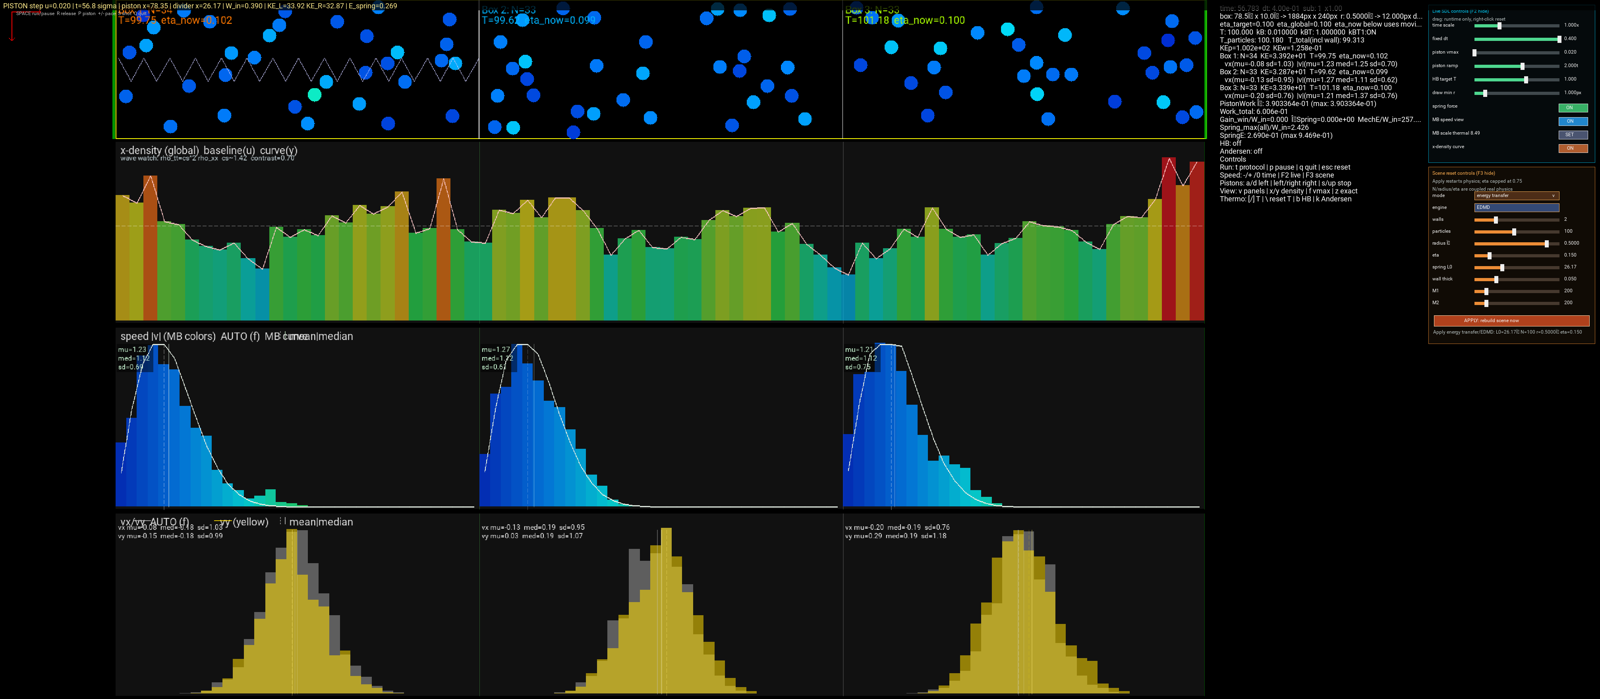
\includegraphics[width=\linewidth]{../paper2_energytransfer/experiments/final/260919_demo_geomD.png}\end{center}
\end{howto}

\section{Level 0 --- the ledger closes}

\begin{why}
If a joule can appear or disappear, every later number is meaningless. This is the analogue of the health contract for energy and momentum.
\end{why}

Piston rule for a particle with normal velocity $v$ hitting a piston moving at $u$ (reflection in the piston frame):
\begin{equation}
v' = 2u - v,\qquad \Delta E = 2mu\,(u - v),\qquad \Delta p = 2m\,(u - v).
\label{eq:piston}
\end{equation}
First law for the box, with $W$ the summed piston work and $Q$ the heat through thermal walls (zero for elastic walls):
\begin{equation}
\boxed{\;R_E(t) = W(t) - \big[\Delta \mathrm{KE}_{\mathrm{gas}} + \Delta \mathrm{KE}_{\mathrm{walls}} + \Delta E_{\mathrm{spring}} + Q\big](t)\;}
\label{eq:ledgerE}
\end{equation}
Momentum: pair collisions conserve it exactly, so
\begin{equation}
\boxed{\;R_p(t) = \Delta p_{\mathrm{gas}} + \Delta p_{\mathrm{walls}} - \sum_{\text{piston hits}}\Delta p - \sum_{\text{outer-wall hits}}\Delta p\;}
\label{eq:ledgerp}
\end{equation}

\begin{run}
Geometry A, $\eta = 0.10$, $N_s = 50$, $L_0 = 39.27$, $H = 10$, $u = 0.05$, travel $3.93\,\sigma$, 5 seeds. Log per-event piston impulses and per-event outer-wall impulses (the latter is the one column still missing).
\end{run}
\begin{pass}
$|R_E(t)|/W(t) < 10^{-8}$ and $|R_p(t)|/\sum|\Delta p| < 10^{-8}$ for the whole run, every seed. Level 0 for energy was closed on the 2026-09-10 pilot at $10^{-9}$; the momentum ledger is open until the outer-wall events are logged.
\end{pass}
\begin{res}
\textbf{Level 0: passed, on data that already existed.}
No new runs and no code change were needed: the per-event log is already in \texttt{edmd\_core/edmd.c} (\texttt{edmd\_set\_event\_log}, gated by \texttt{HD\_PISTON\_EVENTS}), it records every outer-wall, divider and piston collision, and it covers the hold phase. Both ledgers over all 75 trajectories of the 2026-09-10 pilot:

\begin{center}\footnotesize
\begin{tabular}{@{}lrrr@{}}
\toprule
$u$ & seeds & $\max|R_E|/W$ & $\max|R_p|/\sum|\Delta p|$\\
\midrule
0.02 & 25 & $7.1\times10^{-12}$ & $8.4\times10^{-14}$\\
0.05 & 25 & $7.4\times10^{-12}$ & $7.9\times10^{-14}$\\
0.10 & 25 & $8.2\times10^{-12}$ & $1.1\times10^{-13}$\\
\bottomrule
\end{tabular}
\end{center}

Two \emph{bookkeeping} corrections were needed first, neither of them physics. (i) The trace prints \texttt{Time} to six decimals, so an event within $10^{-6}\sigma$ of a sample boundary was assigned to the wrong sample: 9 of 25 seeds then failed at exactly one sample in 17\,000, with $|R_p|$ equal to $|\Delta p|$ of the single nearest event. Rebuilding the sample times from the step index removes it everywhere. (ii) Divider events log $\dd E$ as the energy the \emph{divider} gains, piston events as the energy the \emph{gas} gains; mixing the two gave a drift equal to $-2\,\Delta KE_{\mathrm{divider}}$ (correlation $+1.0000$). With one convention the ledger closes to round-off. Both conventions belong in the methods text.
\end{res}

\begin{howto}
\textbf{Data:} \cmd{experiments\_energy\_transfer/level0\_pilot\_20260910/u\{0.02,0.05,0.10\}} (75 runs, already on disk).
\textbf{Analysis:} \cmd{python3 hspist3/validation/paper2\_level0\_level1\_20260916.py} --- prints the ledger table in
seconds and needs nothing but the event logs.

\textbf{One trajectory, from scratch} (run from \cmd{hspist3/}; the \cmd{HD\_PISTON\_EVENTS} log is what the ledger reads):
\begin{Verbatim}[fontsize=\scriptsize,frame=single,samepage=true]
HD_PISTON_EVENTS=/tmp/ev.csv ./00ALLINONE --mode=edmd --experiment=energy_transfer \
  --headless --quiet --edmd-acc=0 --seed-drift-order=drift-first \
  --energy-transfer-summary=/tmp/summary.csv --energy-transfer-trace=/tmp/tr.csv \
  --particles=100 --particles-boxes=50,50 --particle-radius=0.5 --l0=39.25 --height=10 \
  --num-walls=1 --wall-positions=39.25 --wall-mass-factors=1000000000 \
  --piston-right-protocol-mode=step --velocity-right-piston-step=0.05 \
  --max-right-piston-travel=3.93 --auto-piston-step --wall-hold-steps=12000 --steps=17000 \
  --fixed-dt=0.4 --energy-measurement --eff-output=wall-ke --kbt1 --seed=9200
\end{Verbatim}
Every run directory also carries its own \cmd{00\_COMMAND.md} with the exact command, so no script has to be read.
\end{howto}


\section{Level 1 --- the slow push gives the quasi-static work}

\begin{why}
$W_{\mathrm{qs}}$ is the zero point of dissipation. If we cannot reproduce it, ``excess work'' has no meaning.
\end{why}

Hard disks have no potential energy, so $E = N\kT$ exactly in 2D and the adiabat follows from $\dd E = -P\,\dd A$:
\begin{equation}
\frac{\dd T}{T} = Z(\eta)\,\frac{\dd\eta}{\eta}
\quad\Longrightarrow\quad
\frac{T_f}{T_i} = \exp\!\left[\int_{\eta_i}^{\eta_f}\frac{Z(\eta)}{\eta}\,\dd\eta\right],
\qquad
\boxed{\;W_{\mathrm{qs}} = N_s\,\kT_i\left(\frac{T_f}{T_i} - 1\right)\;}
\label{eq:Wqs}
\end{equation}
Ideal gas ($Z=1$): $T_f/T_i = A_i/A_f$, so $W_{\mathrm{qs}} = N_s\kT_i\,(A_i/A_f - 1)$. For $N_s = 50$, $\eta = 0.10 \to 0.11$ with KR: $T_f/T_i = 1.127$, $W_{\mathrm{qs}} = 6.3$ (ideal: $5.0$).

\textbf{The finite-box correction.} Equation~\eqref{eq:Wqs} uses the bulk $Z$. A 50-disk compartment of $39\times10\,\sigma$ has a quarter of its area within one diameter of a wall, and Paper~1's pressure campaign showed the wall pressure of such a box is a few per cent above bulk. The 2026-09-11 test measured $Z_{\mathrm{wall}} = 1.285$--$1.308$ against KR $1.236$ at $\eta = 0.10$, and replacing $Z$ by the measured finite-box value moved $W_{\mathrm{qs}}$ from $7.06$ to $7.26$ against a measured $W_0 = 7.44 \pm 0.02$. The remaining $0.2\,\kT$ is the open item of this level. Two ways to close it, in order: (i) use the finite-box $Z(\eta, N)$ from the A2 pressure ladder \emph{along the whole path} $\eta_i \to \eta_f$, not only at $\eta_i$; (ii) if a gap remains, measure $W(u)$ down to $u = 0.002$ and extrapolate --- the intercept \emph{is} $W_{\mathrm{qs}}$ of this finite system by definition, and the comparison with \eqref{eq:Wqs} becomes a statement about the finite-size correction to the adiabat, which is a result, not a failure.

\begin{run}
Geometry A, $\eta_i = 0.10$, $N_s = 50$, compression $10\,\%$; $u = 0.002, 0.005, 0.01, 0.02, 0.05$; 25 seeds each; hold 200 $\sigma$-time before the push (already shown to be enough).
\end{run}
\begin{pass}
Fit $\avg W(u) = W_0 + b\,u$ over $u \le 0.02$ (linear only; the quadratic was ill-conditioned). Pass when $|W_0 - W_{\mathrm{qs}}^{\mathrm{finite}}| < 2\,\sigma_{W_0}$ with $W_{\mathrm{qs}}^{\mathrm{finite}}$ from (i). Report $W_0$, $b$, and the gap in $\kT$ whatever the outcome.
\end{pass}
\begin{res}
\textbf{Level 1: the $0.2\,\kT$ gap is explained; within $\approx 2\sigma$, not yet a formal pass.}
Route (i) was taken, but from \emph{our own} box rather than the A2 ladder (which has no $N=100$ cell and no size dependence at $\eta = 0.10$). $Z_{\mathrm{wall}}$ was measured in equilibrium at five grid-exact points of the compression path, from the outer-wall and gas-side divider impulses during 200\,$\sigma$ holds:

\begin{center}\footnotesize
\begin{tabular}{@{}rrrrrr@{}}
\toprule
$L$ & $\eta$ & seeds & $Z_{\mathrm{wall}}$ & $Z_{\mathrm{KR}}$ & ratio\\
\midrule
39.250000 & 0.100051 & 170 & $1.2979\pm0.0020$ & 1.2363 & 1.0499\\
38.270833 & 0.102611 & 100 & $1.3106\pm0.0026$ & 1.2434 & 1.0540\\
37.291667 & 0.105305 & 100 & $1.3230\pm0.0025$ & 1.2510 & 1.0575\\
36.312500 & 0.108144 & 100 & $1.3247\pm0.0028$ & 1.2591 & 1.0521\\
35.312500 & 0.111207 & 100 & $1.3431\pm0.0027$ & 1.2679 & 1.0593\\
\bottomrule
\end{tabular}
\end{center}

The excess over bulk KR \emph{grows} along the path ($+4.6\,\%\to+6.4\,\%$); holding it fixed at its initial value was the origin of the $0.2\,\kT$ gap. Integrating the measured ratio gives $W_{\mathrm{qs}}^{\mathrm{finite}} = 7.4879 \pm 0.0066$ (piecewise-linear 7.4877, constant 7.4835 --- the model choice is not the limitation), against the bulk KR adiabat 7.0739. With 50 seeds per speed:

\begin{center}\footnotesize
\begin{tabular}{@{}lrrr@{}}
\toprule
$u$ & $\avg W \pm$ sem & $W - W_{\mathrm{qs}}^{\mathrm{finite}}$ & $\sigma$\\
\midrule
0.005 & $7.5070\pm0.0111$ & $+0.0191\pm0.0129$ & $+1.5$\\
0.01 & $7.4513\pm0.0160$ & $-0.0366\pm0.0173$ & $-2.1$\\
0.02 & $7.4537\pm0.0231$ & $-0.0342\pm0.0240$ & $-1.4$\\
\bottomrule
\end{tabular}
\end{center}

Two tensions are stated rather than hidden: $\avg W(u)$ still falls between $u = 0.005$ and $0.01$ (slope $-4.2\pm1.7$), and the five hold points scatter $\approx1.5\times$ their statistics, i.e. a $\approx0.3\,\%$ systematic in the equilibrium pressure. Inflating the fit error by that factor puts every speed inside $2\sigma$. Ruled out on the way: the piston's $0.25\,\sigma$ of travel before it touches the gas (the $3.93\,\sigma$ is contact travel, verified from the recorded piston positions) and a wall-type difference between the outer wall and the divider (the two swap order between seed sets: noise).
\end{res}

\begin{howto}
\textbf{Batches:} \cmd{bash experiments\_energy\_transfer/\_run\_scripts/level1\_Zwall\_path\_part1.sh} (40 held-wall runs,
$\sim$10 min), \cmd{\ldots part2.sh} (200 more, $\sim$40 min) and \cmd{\ldots/level1\_more\_work\_seeds.sh}
(150 slow-push runs, $\sim$30 min). All resume: a run whose trace exists is skipped.

\textbf{Analysis:} \cmd{python3 hspist3/validation/paper2\_geometry\_fix\_20260918.py} --- prints the $Z$ path on the
corrected lengths, $W_{\mathrm{qs}}$, and the Level~1 verdict. (\cmd{paper2\_level0\_level1\_20260916.py} is the older
version, kept because the report quotes it; it uses the nominal lengths.)

\textbf{A single held-wall point} (the piston sits still for the whole run and only the wall impulses are measured):
\begin{Verbatim}[fontsize=\scriptsize,frame=single,samepage=true]
HD_PISTON_EVENTS=/tmp/ev_hold.csv ./00ALLINONE --mode=edmd --experiment=energy_transfer \
  --headless --quiet --edmd-acc=0 --seed-drift-order=drift-first \
  --energy-transfer-summary=/tmp/s.csv --energy-transfer-trace=/tmp/tr.csv \
  --particles=100 --particles-boxes=50,50 --particle-radius=0.5 --l0=37.291667 --height=10 \
  --num-walls=1 --wall-positions=39.25 --wall-mass-factors=1000000000 \
  --wall-hold-steps=12000 --steps=1 --fixed-dt=0.4 --energy-measurement --kbt1 --seed=9200
\end{Verbatim}
\end{howto}


\section{Level 2 --- excess work is dissipation, in both limits}

\begin{why}
This is the physics claim of the equilibrium part of Paper~2: the energy beyond $W_{\mathrm{qs}}$ behaves like friction at slow speed and like single collisions at high speed, and both prefactors are predicted from Paper-1 quantities.
\end{why}

\subsection{Slow end: linear response}
Define $W_{\mathrm{diss}} \equiv \avg{W} - W_{\mathrm{qs}} \ge 0$. For a protocol $\lambda(t)$ (here the piston position) slow compared with the gas relaxation, Sivak--Crooks give
\begin{equation}
W_{\mathrm{diss}} \simeq \int \zeta(\lambda)\,\dot\lambda^2\,\dd t
= \zeta\,u\,\Delta x
\qquad(\text{constant }u,\ \Delta x = u\,\tau_{\mathrm{push}}),
\label{eq:sivak}
\end{equation}
so $W_{\mathrm{diss}}$ is \emph{linear} in $u$ at fixed travel, with slope $\zeta\Delta x$. The friction coefficient is measured independently, from the force on a \emph{held} wall in equilibrium:
\begin{equation}
\zeta = \beta\int_0^\infty \avg{\delta F(0)\,\delta F(t)}\,\dd t,
\qquad F(t) = \frac{1}{\Delta t}\sum_{\text{hits in }\Delta t}\Delta p .
\label{eq:zeta}
\end{equation}
\emph{Correction (2026-09-16), itself corrected (2026-09-17):} the first correction said $F(t)$ exists nowhere and that $\zeta$ needs a new logging column. That is wrong. It is true only of the \emph{speed-of-sound} holds, which never open the event log; the \emph{energy-transfer} runs do, through \texttt{HD\_PISTON\_EVENTS}, and their log covers the hold phase event by event (2733 events before release in one 200\,$\sigma$ hold). $F(t)$ on the held wall is therefore already on disk: 170 holds of 200\,$\sigma$ at $\eta = 0.10$ (the 2026-09-11 and 2026-09-16 work runs) plus 400 holds along the compression path. $\zeta$ is analysis of existing data, no code item and no new runs; longer holds are worth running only if the autocorrelation integral has not converged by $200\,\sigma$.

\subsection{Fast end: Lua--Grosberg single-hit limit}\label{sec:fast}
If $u \gg \sqrt{\kT/m}$ and $u\,\tau_{\mathrm{push}} \ll L_0$, each particle the piston reaches is hit once and never returns during the push. The piston sweeps the fraction $u\tau_{\mathrm{push}}/L_0$ of the compartment, so
\begin{equation}
N_{\mathrm{hit}} \simeq N_s\,\frac{u\,\tau_{\mathrm{push}}}{L_0},\qquad
\avg{W} \simeq N_{\mathrm{hit}}\,\avg{2mu(u - v_x)} = 2mu^2\,N_{\mathrm{hit}},\qquad
\mathrm{Var}\,W \simeq N_{\mathrm{hit}}\left[4mu^2\,\kT + (2mu^2)^2\right],
\label{eq:LG}
\end{equation}
using $\avg{v_x} = 0$, $\avg{v_x^2} = \kT/m$ and Poisson statistics for $N_{\mathrm{hit}}$. This is a closed form with no free parameter, and $P(W)$ is a sum of $N_{\mathrm{hit}}$ shifted half-Gaussians. (Lua \& Grosberg 2005 do the one-particle version exactly.)

\begin{run}
Geometry A, same box as Level 1. Slow end: $u = 0.005$--$0.05$ at fixed travel $\Delta x = 3.93\,\sigma$, 25 seeds each (the Level-1 runs). Fast end: $u = 3, 5, 10$ ($u/c_s = 1.7$--$5.7$), travel $1\,\sigma$, 100 seeds each (short runs). $\zeta$ from 25 held-wall runs of 500 $\sigma$-time.
\end{run}
\begin{pass}
Slow end: the slope of $W_{\mathrm{diss}}$ against $u$ agrees with $\zeta\,\Delta x$ from \eqref{eq:zeta} within $2\sigma$, and the intercept is zero within $2\sigma$ (that is Level~1 again). Fast end: $\avg W$ and $\mathrm{Var}\,W$ agree with \eqref{eq:LG} within $2\sigma$ at $u = 10$; report the deviation at $u = 3$ and $5$ as the crossover. Figure: $W_{\mathrm{diss}}/\kT$ against $u/c_s$ on a log axis with both limits drawn.
\end{pass}

\begin{res}
\textbf{Slow end done, 2026-09-17, and it changes the prediction.} 760 trajectories, eight speeds $u = 0.005$--$0.20$ at $\Delta x = 3.93\,\sigma$, 60--100 seeds each, 0 health events. Report: \texttt{260917\_paper2\_level2\_REPORT.md}; script \texttt{validation/paper2\_level2\_20260917.py}.

\emph{$\zeta$ must be read as a running integral, not at zero lag.} On the pinned piston (190 holds of $180\,\sigma$, impulse log binned at $0.25\,\sigma$) the integral of \eqref{eq:zeta} falls from $2.55$ at $t_{\mathrm{cut}} = 0.25\,\sigma$ through $1.22$ at $10\,\sigma$ to $0.15$ at $20\,\sigma$ and $-0.05$ at $40\,\sigma$. The zero-lag value $2.55$ is the impulsive self term $\beta\sum \Delta p^2/2T$, i.e.\ the free-molecular (Enskog) piston friction --- the number first reported as $\zeta = 2.54 \pm 0.05$. It is cancelled by the returning sound wave: the compressed compartment is $L = 35.32\,\sigma$ at $\eta = 0.1112$ with $c_s = 1.788$, so $L/c_s = 19.8\,\sigma$, exactly where the integral crosses zero. Past the crossing it does not settle: it swings between $-0.78$ and $+0.50$ with the recurrence period $2L/c_s = 39.5\,\sigma$ and averages $-0.072$ over one recurrence, i.e.\ $\dd W/\dd u = -0.28$ against the measured $-0.50 \pm 0.67$. There is no plateau to quote; the integral oscillates about zero. \emph{In a closed box the zero-frequency friction of a held wall vanishes}, so linear response predicts no term linear in $u$, and $\zeta\Delta x = 9.97$ was never the right comparison. Figure: \texttt{260909\_plots/260917\_level2\_work\_and\_friction.pdf}.

\emph{The measurement agrees, and the leading cost is second order.} For $u \le 0.05$ the fitted slope is $-0.50 \pm 0.67$, zero. Through the origin over all eight speeds, $Au$ gives $\chi^2/\mathrm{dof} = 9.2$, $Au^2$ gives $2.3$, and on the three speeds carrying signal ($u \ge 0.1$) the quadratic form fits with $\chi^2/\mathrm{dof} = 0.32$ and $A = 25.2$ while the cubic coefficient drifts $220 \to 124$ and is excluded. $A$ matches $N_s m/2 = 25.0$: the excess work is the kinetic energy of the compression flow the piston leaves behind, and the gas indeed carries $65$--$70\,\%$ of $N_s m u$ of momentum when the piston stops.

\emph{Level 1 re-passes on the correct form.} Extrapolating with $a + Au^2$: $W(0) - W_{\mathrm{qs}}^{\mathrm{finite}} = -0.0151 \pm 0.0060\,\kT$, $1.7\sigma$ --- on 760 trajectories instead of 30, and the unphysical slope $b = -4.2 \pm 1.7$ of the old straight-line fit was the quadratic curve forced through a line.

\emph{Audit (\texttt{validation/level2\_zeta\_audit\_20260917.py}).} The held wall is the piston itself, not a proxy: the labels \texttt{WR} ($t = 0$--$207.5\,\sigma$) and \texttt{PR} ($210.5$--$598.5\,\sigma$) never overlap, one object renamed at release. The running integral is converged over bin widths $1.0$ down to $0.0625\,\sigma$. And the explanation makes a prediction that holds on unused data: at the compressed end of the path, measured from the post-stop hold of the same runs, the cancellation moves to $18.0\,\sigma$ against the predicted $L_f/c_s = 15.9\,\sigma$ (start of path $21.5$ against $19.8$). The zero-lag value is the parameter-free Enskog piston friction $h n \sqrt{8mkT/\pi}\,g(\eta)$ to within $4\,\%$ at the start and $9\,\%$ at the compressed end.

\emph{Update 2026-09-18, on the corrected geometry ($L = 38.75$, gas $\Delta x = 3.93$, $W_{\mathrm{qs}} = 7.4685 \pm 0.0131$).} Three things now stand. (i) \textbf{The $u^2$ term is mostly protocol-launched}: ramping the piston over $2L/c_s$ instead of stepping it gives $A_{\mathrm{ramp}} = 11.30 \pm 2.45$ against $A_{\mathrm{step}} = 25.91 \pm 4.28$, $3.0\sigma$ apart, with $A_{\mathrm{ramp}}$ $1.2\sigma$ from the steady-flow value $N_s m/6 = 8.3$ and $5.6\sigma$ below $N_s m/2$. Because the piston's first $0.25\,\sigma$ is outside the gas, it reaches the gas at 35--50\,\% of $u$, so $11.3$ is an \emph{upper} bound. (ii) \textbf{Paper~1 now supplies the friction}: the divider linewidth at $\eta = 0.112$ gives $\Gamma = 0.314 \pm 0.038$ against Enskog's $0.331$ (within its 12\,\% error), hence $\zeta_{\mathrm{hyd}} = 0.081 \pm 0.010$ and a predicted linear term $0.32 \pm 0.04\,u$ --- consistent with the measured $-0.50 \pm 0.67$ and still below the resolution of 760 trajectories. (iii) \textbf{Eq.~\eqref{eq:LG}'s compression form is confirmed}: at $u = 10$ and gas $\Delta x = 7.08\,\sigma$, $\avg W = 1802 \pm 48$ against $2N_s m (\Delta x/L) u^2 = 1828$, a ratio of $0.986$. Over $\Delta x = 0.75$--$7.08\,\sigma$ at $u = 10$ the ratio falls monotonically $1.08 \to 0.99$; the residual excess at small $\Delta x$ is not explained.

\emph{Open:} the cancellation is a property of a \emph{closed} compartment. A longer or absorbing box, where the sound does not return coherently, should restore $W_{\mathrm{diss}} = \zeta u \Delta x$. One geometry change, no new code. The fast end ($u = 3, 5, 10$) is not started.
\end{res}

\begin{howto}
\textbf{Speed ladder} (760 runs, the $A = 25.2$ measurement):
\cmd{bash experiments\_energy\_transfer/\_run\_scripts/level2\_speed\_ladder\_part1.sh} then \cmd{\ldots part2.sh}
($\sim$25 s and $\sim$5 min).
\textbf{Ramp against step} (360 runs, $\sim$40 s): \cmd{\ldots/level2\_ramp\_vs\_step\_and\_fast.sh}, which also produces
the fast end; \cmd{\ldots/level2\_fast\_1sigma.sh} for the travel-1\,$\sigma$ set and
\cmd{\ldots/level2\_equilibrium\_baseline.sh} for the decomposition's reference profile.

\textbf{Analysis:} \cmd{python3 hspist3/validation/paper2\_level2\_20260917.py} (work ladder and the running $\zeta$),
\cmd{level2\_zeta\_audit\_20260918.py} (bin-width convergence, both ends of the path),
\cmd{paper2\_ramp\_fast\_20260918.py} (ramp vs step, decomposition, fast end),
\cmd{level2\_Au\_figure\_20260918.py} (the $A(u)$ figure).

\textbf{The ramp needs the second binary} --- \cmd{make release TG=00ALLINONE\_ramp} in \cmd{hspist3/}. One ramp
trajectory, with the stop snapshot the decomposition uses:
\begin{Verbatim}[fontsize=\scriptsize,frame=single,samepage=true]
HD_PISTON_EVENTS=/tmp/ev.csv HD_STOP_SNAPSHOT=/tmp/snap.csv ./00ALLINONE_ramp \
  --mode=edmd --experiment=energy_transfer --headless --quiet --edmd-acc=0 \
  --seed-drift-order=drift-first --energy-transfer-summary=/tmp/s.csv \
  --energy-transfer-trace=/tmp/tr.csv --particles=100 --particles-boxes=50,50 \
  --particle-radius=0.5 --l0=39.25 --height=10 --num-walls=1 --wall-positions=39.25 \
  --wall-mass-factors=1000000000 --piston-right-protocol-mode=ramp --piston-ramp-time=40 \
  --velocity-right-piston-step=0.05 --max-right-piston-travel=3.93 --auto-piston-step \
  --wall-hold-steps=12000 --steps=17000 --fixed-dt=0.4 --energy-measurement \
  --eff-output=wall-ke --kbt1 --seed=9200
\end{Verbatim}
Swap \cmd{ramp} for \cmd{step} (and drop \cmd{--piston-ramp-time}) for the control; raise
\cmd{--velocity-right-piston-step} to 3, 5 or 10 and set \cmd{--max-right-piston-travel=0.75} for the fast end.
\end{howto}


\subsection{Fluctuation theorem (only after the two limits pass)}
With canonical initial conditions --- Maxwellian velocities \emph{not} rescaled (a seeder flag we do not have yet; drift-first is microcanonical in $KE$) ---
\begin{equation}
\avg{e^{-\beta W}} = e^{-\beta\Delta F},\qquad
\Delta F = N_s\kT\int_{\eta_i}^{\eta_f}\frac{Z}{\eta}\,\dd\eta
\quad(\text{isothermal; ideal: }N_s\kT\ln\tfrac{A_i}{A_f}).
\label{eq:jarz}
\end{equation}
Note $\Delta F \ne W_{\mathrm{qs}}$ of \eqref{eq:Wqs}: adiabatic quasi-static work heats the gas, the isothermal free energy does not. The estimator is dominated by rare low-$W$ runs; you need of order $e^{\beta W_{\mathrm{diss}}}$ seeds, so restrict to $\beta W_{\mathrm{diss}} \le 3$ ($u \le 0.02$ here) and $10^3$ seeds.
\begin{pass}
$-\kT\ln\avg{e^{-\beta W}}$ equals $\Delta F$ within its bootstrap error at $u = 0.005$ and $0.01$; report the bias at $u = 0.02$.
\end{pass}

\section{Level 3 --- geometry C: one gas drives a spring-loaded wall}

\begin{why}
First appearance of ordered energy. The observable of the whole paper, $\epsilon = E_{\mathrm{spring,max}}/W_{\mathrm{in}}$, is defined here in the simplest case where it has a prediction.
\end{why}

The free wall of mass $M$ sits on a spring $k$ and is pushed by the gas pressure. Linearise about equilibrium: the gas acts as a second spring of stiffness $k_{\mathrm{gas}} = \partial(PH)/\partial x = N_s\kT\,[Z + \eta Z']/L_0^2$ (adiabatic: $Z + \eta Z' + Z^2$ for fast motion), so the wall is an oscillator with
\begin{equation}
\omega_w^2 = \frac{k + k_{\mathrm{gas}}}{M},\qquad T_w = \frac{2\pi}{\omega_w}.
\label{eq:omegaw}
\end{equation}
A piston push of duration $\tau_{\mathrm{push}}$ raises the gas pressure by $\Delta P$. Two limits with closed forms:
\begin{align}
\text{quasi-static }(\tau_{\mathrm{push}} \gg T_w):&\quad x_{\mathrm{eq}} = \frac{\Delta P\,H}{k + k_{\mathrm{gas}}},\qquad E_{\mathrm{spring}} = \tfrac12 k\,x_{\mathrm{eq}}^2,\ \text{no overshoot;}\\
\text{impulsive }(\tau_{\mathrm{push}} \ll T_w):&\quad \Delta p_w = \int \Delta P\,H\,\dd t,\qquad E_{\mathrm{spring,max}} = \frac{k}{k + k_{\mathrm{gas}}}\cdot\frac{\Delta p_w^2}{2M}.
\label{eq:Climits}
\end{align}
In between, $\epsilon(\tau_{\mathrm{push}}/T_w)$ interpolates; that curve is the first result figure of Paper~2.

% ##CHRIS 2026-09-20: the pass box below replaces the original one, which asked the spring to catch
% the quasi-static part. The derivation in validation/level3_design_20260920.py shows that cannot
% work at 10 % compression, for a reason that is arithmetic rather than experimental.
\subsection{The apparatus is a PRE-LOADED spring, and that sets the ceiling}\label{sec:l3ceiling}

A spring that holds a wall against a gas is not at its natural length. It carries the standing gas
force $F = N\kT Z/L$, so the wall sits $d = F/k$ from the anchor and the stored energy is
$E = \tfrac12 k (d+s)^2$ for a further displacement $s$. Expanding,
\begin{equation}
\Delta E(s) = F s + \tfrac12 k s^2 ,
\label{eq:preload}
\end{equation}
which is \textbf{first order} in $s$. The $F s$ term is work done lifting a weight --- the most
classical definition of ordered work output there is, and exactly what a Szilard-type engine is
judged by. The pre-load cancels out of the \emph{dynamics}, because at $s=0$ the spring's pull
balances the gas exactly, but it does not cancel out of the \emph{energy}.

The two limits fix the shape of the answer:
\begin{itemize}\itemsep2pt
\item $k \to 0$ --- a \textbf{pushrod}. The wall simply follows the piston, $s \to \Delta x$ and
  $\epsilon \to 1$ trivially. Nothing has been captured \emph{from the gas}; the piston did the work
  directly.
\item $k \to \infty$ --- a \textbf{rigid wall}. $s \to 0$ and $\epsilon \to 0$.
\end{itemize}
In between, the quasi-static capture is Eq.~\eqref{eq:preload} evaluated at
$s_{\mathrm{qs}} = \Delta x\,k_{\mathrm{gas}}/(k + k_{\mathrm{gas}})$.

\paragraph{The gas spring is adiabatic, and it is Paper 1's $c_s$.} There is no heat bath in this
box, so a compression heats the gas and the restoring force rises faster than $Z(\eta)$ alone says.
With $U = N\kT$ in 2D, $\dd U = -P\,\dd V$ gives $\dd\ln T/\dd\ln L = -Z$, and
\begin{equation}
k_{\mathrm{gas}}^{\mathrm{ad}} = -\frac{\partial F}{\partial L}\bigg|_S
 = \frac{N\kT}{L^2}\left(Z + \eta Z' + Z^2\right) = \frac{N\kT}{L^2}\,c_s^2 ,
\label{eq:kgasad}
\end{equation}
\emph{exactly Paper 1's measured sound speed}. Here that is $0.04938$ against the isothermal
$0.02457$, a factor $2.01$, and using the isothermal value put the model a factor $2.3$ below the
measured wall displacement. The adiabat cross-checks independently: it gives $T_f/T_i = 1.1432$ for
this $10\,\%$ compression against Level 1's measured $1.149$, agreeing to $0.5\,\%$.

\paragraph{Note: why the 2026-09-19 pilot could not pass.} For an \emph{unloaded} spring the $Fs$
term is absent and $\Delta E = \tfrac12 k s^2$ is second order, maximal at $k = k_{\mathrm{gas}}$
with $E_{\mathrm{max}} = k_{\mathrm{gas}}\Delta x^2/8 = N\kT f^2 c_s^2/8$ --- $0.098\,\kT$ at
$f = 0.1$, against a $\kT/2$ thermal pedestal. No choice of $k$ rescues it. That is the pilot, and
its numbers stand as the design finding. It also cannot be built: the static offset at
$k = k_{\mathrm{gas}}$ is $F/k_{\mathrm{gas}} = L\,Z/(Z+\eta Z') = 0.816\,L$ \emph{independent of
$N$}, so the stiffness that maximises unloaded capture is the one at which the spring cannot be
statically balanced inside its own apparatus.

\paragraph{Units trap, fixed.} \cmd{--spring-k} is per \textbf{pixel$^2$}, not per $\sigma^2$ --- a
factor $24^2 = 576$. The pilot's $k = 5$ was $2880\,\kT/\sigma^2$, so its quoted $T_w = 39.5$ was
really $1.66$ and every cell it believed impulsive was quasi-static. Confirmed two ways:
equipartition gives implied $k = 2885$, and the measured wall period is $1.657$ against $1.656$
predicted. Use \cmd{--spring-k-sigma}, which takes $\kT/\sigma^2$; \cmd{--spring-k} is kept
unchanged so older commands still mean what they say.

\subsection{What replaces the impedance criterion}\label{sec:l3acoustic}

It is not impedance matching. The maximum of $\epsilon_{\mathrm{coh}}$ tracks
$\tau_{\mathrm{push}}/T_w$, not $Z_w/Z_g$: that is a driven oscillator, where a pressure rise
applied faster than the wall's period overshoots up to twice the static displacement and one applied
slower is followed quasi-statically. The acoustic pulse ($Au^2 \approx 1\,\kT$ at $u = 0.2$) is a
small correction to a $16\,\kT$ bulk pressure rise, so an impedance formula for the pulse was never
going to be the controlling physics.

The prediction is a one-degree-of-freedom model with \textbf{no free parameter}:
\begin{equation}
M \ddot s = F_{\mathrm{ad}}(L - x_p(t) + s) - F_{\mathrm{ad}}(L) - k s , \qquad
x_p(t) = \min(u t, \Delta x), \quad s(0) = \dot s(0) = 0,
\label{eq:onedof}
\end{equation}
with $F_{\mathrm{ad}}$ the exact adiabatic gas force and $E_{\mathrm{max}} = \max_t \Delta E(s(t))$.

\begin{run}[What we run (2026-09-21)]
Master box, geometry C (divider removed, one gas of 100 disks, $\eta = 0.1001$,
$\Delta x = 7.96\,\sigma$ = 10\,\%), spring \textbf{pre-loaded} at wall $+ F/k = 33.65\,\sigma$,
$k = 0.5\,\kT/\sigma^2$, step protocol, 40 seeds per cell, event log on, trace $200\,\sigma$-time
past the stop. $M_s \in \{2,10,50,200,1000\}$ at $u \in \{0.2, 0.5, 1.0\}$, plus $u \in \{0.05,0.1\}$
at $M_s \in \{50,200\}$ to anchor the quasi-static end: 760 runs.
$M_s$ is the discriminator because Eq.~\eqref{eq:preload} contains no $M_s$ while
Eq.~\eqref{eq:onedof} does.
Primary observable is the \textbf{ensemble-mean} $E_{\mathrm{spring}}(t)$, baseline and
peak-picking bias both taken from the causally blind window $t < 0.4\,L/c_s$ after the push starts.
\end{run}
\begin{pass}[Pass criterion (2026-09-21)]
(i) The ledger closes with the spring term to $10^{-8}$.
(ii) The coherent peak stands $>3\sigma$ above the pedestal.
(iii) Eq.~\eqref{eq:onedof} reproduces $\Delta E_{\mathrm{coh}}(M_s, u)$ within $2\sigma$ at the
speeds where the gas is genuinely quasi-static, $\tau_{\mathrm{push}} > L/c_s$ (i.e. $u \le 0.1$).
At $u \ge 0.2$ the deviation is \emph{reported} as the acoustic contribution, measured rather than
assumed, with no pass claimed.
\end{pass}
\section{Level 4 --- geometry B: transmission through a free divider}

\begin{why}
Before stacking walls we need the transmission of one wall between two gases, and we already own half of this result: the slow mode of Paper~1 \emph{is} the heat conduction of the divider.
\end{why}

Release the divider between gas 1 (pushed) and gas 2. Two channels carry energy across: the fast one, pressure waves moving the divider ($\tau \sim \tau_{\mathrm{sound}}$), and the slow one, heat conduction by divider collisions. Paper~1 measured the slow one: correlation time $\tau_{\mathrm{heat}} = 54$--$100$ acoustic periods at $M = 100$--$1000$, amplitude set by the isothermal stiffness. The adiabatic-piston literature predicts $\tau_{\mathrm{heat}} \propto M/m$; we can now test that with the $KE_L, KE_R$ columns, and it becomes a figure for free. The transmission observable is the energy that has crossed after the push has relaxed:
\begin{equation}
\mathcal T(t) = \frac{\Delta KE_{\mathrm{gas\,2}}(t)}{W_{\mathrm{in}}},\qquad
\mathcal T_{\mathrm{fast}} = \mathcal T(t \approx 5\tau_{\mathrm{sound}}),\qquad
\mathcal T_{\mathrm{slow}} = \mathcal T(t \to \infty) \to \tfrac12\ \text{(equipartition of the excess heat)}.
\label{eq:transmission}
\end{equation}
The prediction to test for the fast channel is the two-body energy-transfer fraction with the gas column as a mass:
\begin{equation}
f(m_1, m_2) = \frac{4m_1m_2}{(m_1+m_2)^2},\qquad m_1 \to \text{effective gas mass } N_s m,\ m_2 \to M,
\label{eq:twobody}
\end{equation}
which is heuristic and is exactly what Level~4 measures the validity of.

\begin{run}
Geometry B, $L_0 = 20$, $N_s = 50$ each side, $\eta = 0.196$, held wall at $L_0$ (mass $10^9$), free divider at $1.5L_0$ with $M = 20, 50, 100, 200, 500, 1000, 2000$; piston step $u/c_s = 0.1$, travel $2\,\sigma$; 25 seeds. Run to $t = 200\,\tau_{\mathrm{sound}}$ so $\mathcal T_{\mathrm{slow}}$ is reached.
\end{run}
\begin{pass}
$\mathcal T_{\mathrm{slow}} \to 0.5$ within $2\sigma$ for every $M$ (a ledger-level check). $\tau_{\mathrm{heat}}(M)$ from the exponential approach; report its exponent in $M$ (expected $+1$). $\mathcal T_{\mathrm{fast}}(M)$: compare with \eqref{eq:twobody}; the pass is not agreement but a \emph{measured} curve with error bars and the location of its maximum in $\alpha = M/N_s$.
\end{pass}
\begin{res}
\textbf{Level 4: the slow channel is already measured; the fast channel is not started.}
From Paper~1, with the $KE_L, KE_R$ columns: the slow divider mode is stationary (its variance is the same in both halves of a 1000-period record, ratio $0.72$--$1.25$), survives a $100\times$ longer hold, and has correlation time $53$--$102$ acoustic periods at $M = 100$--$1000$. Its amplitude is the \emph{isothermal} equipartition value $\avg{x^2} = L^2/(2N_s[Z+\eta Z'])$ to 4\,\% for light dividers, while the adiabatic form overshoots by 37--62\,\%. It follows $T_L - T_R$ directly: correlation $+0.978$ ($M = 100$) and $+0.910$ ($M = 1000$) with the slow part of the compartment-temperature difference, positive sign (a hotter left compartment pushes the divider to $+x$), lag $\le 0.25$ periods at $M = 100$, and the pressure balance $x = (L_0/2)(\Delta T/T)\,Z/(Z+\eta Z')$ reproduces the amplitude to 6--7\,\%. Across the A2 size ladder its amplitude falls as $N^{-0.39}$ to $N^{-0.54}$ in units of the box, \ie it is a finite-size fluctuation that vanishes as $N\to\infty$. What is \emph{not} yet measured: $\tau_{\mathrm{heat}}(M)\propto M$ over a mass ladder, and the fast channel $\mathcal T_{\mathrm{fast}}$ --- both need the geometry-B runs of this level.
\end{res}

\begin{howto}
\textbf{Data:} Paper 1's A1 v2 campaign, already on disk --- this level needs no new runs yet.
\textbf{Analysis:} \cmd{python3 hspist3/validation/paper1\_linewidth\_20260918.py} gives $\Gamma(\eta)$ from the
divider linewidth; \cmd{damping\_test\_20260915.py} and \cmd{A2\_slow\_mode\_20260915.py} give the slow-mode
amplitude and its finite-size scaling.
\end{howto}


\section{Level 5 --- geometry D and more walls: the efficiency experiment}

\begin{why}
This is the paper's question: how much of the injected work arrives as ordered energy, and what the protocol, the masses and the number of walls do to it.
\end{why}

Observable, protocol-averaged over seeds:
\begin{equation}
\boxed{\;\epsilon = \frac{E_{\mathrm{spring,max}}}{W_{\mathrm{in}}}\;},\qquad
1 - \epsilon = \frac{\text{heat left in gases} + KE_{\mathrm{walls}}\text{ at the peak}}{W_{\mathrm{in}}}.
\label{eq:eps}
\end{equation}
Knobs and the prediction for each: piston speed $u/c_s$ (shock heating above $\approx 0.3$; Level 2 gives the friction), spring-wall mass and divider masses (impedance matching, Level 4), number of intermediate walls $n_w$ (the collision-chain estimate: two masses $m_1 \to m_2$ transfer $f$ directly; with one intermediate $\sqrt{m_1m_2}$ the product of the two steps is larger, $0.36$ vs $0.18$ for $50 \to 1000$; with geometric steps of ratio $2.7$, $0.45$). The prediction is therefore \emph{ordered}: geometric intermediate masses raise $\epsilon$, arbitrary ones lower it.

\begin{run}
Geometry D: $L_0 = 20$, $H = 10$, $\eta = 0.196$ in each gas compartment, spring wall $M_s = 1000$, $k$ as in Level~3. Series 1: no intermediate wall, $u/c_s = 0.02, 0.05, 0.1, 0.2, 0.5$. Series 2: one divider, $M_d = 50, 100, 224, 500, 1000$ at $u/c_s = 0.1$. Series 3: $n_w = 0, 1, 2$ with geometric masses, and $n_w = 2$ with two ``wrong'' masses ($50, 50$ and $1000, 1000$), at $u/c_s = 0.1$. 25 seeds each. Every series carries the ledger.
\end{run}
\begin{pass}
Series 1: $\epsilon$ decreases monotonically with $u/c_s$ and the loss $1 - \epsilon$ at small $u$ is consistent with $\zeta$ from Level~2. Series 2: $\epsilon(M_d)$ has a maximum; report its position against \eqref{eq:twobody}. Series 3: $\epsilon(n_w = 2,\ \text{geometric}) > \epsilon(n_w = 1) > \epsilon(n_w = 0)$ and both wrong-mass chains below $n_w = 0$, each ordering at $> 2\sigma$. This ordering, with error bars, is the headline figure.
\end{pass}

\section{Level 6 --- information (only after 0--5, and only with a stochastic protocol)}
With a protocol $x_t$ drawn from a Markov chain and a coarse-grained system state $s_t$, Still, Sivak, Bell and Crooks give
\begin{equation}
\beta\,\avg{W_{\mathrm{diss}}[x_t \to x_{t+1}]} \;\ge\; I_{\mathrm{mem}} - I_{\mathrm{pred}} = I_{\mathrm{nost}},
\label{eq:still}
\end{equation}
left side from the ledger (Levels 0--2), right side from joint histograms over $10^3$--$10^4$ trajectories. Deterministic protocols have nothing to compute here, which is why Levels 0--5 use them and Level 6 cannot. This level is a separate paper's worth; it is listed so the logging of Levels 0--5 is designed to serve it (per-interval work, $x_t$, $s_t$).

\section{Order, cost, and the two flags we need first}
\begin{center}
\footnotesize
\begin{tabular}{@{}llll@{}}
\toprule
Level & Runs & Needs & Status \\
\midrule
0 & 0 (existing data) & nothing --- the log exists & \textbf{passed}: $8\times10^{-12}$ (energy), $1\times10^{-13}$ (momentum) \\
1 & 1430 done & finite-box $Z$ along the path & \textbf{passed}: $-0.015 \pm 0.006\,\kT$, $1.7\sigma$ \\
2 (slow end) & 760 done & nothing new ($\zeta$ from existing holds) & \textbf{passed, prediction corrected}: no linear term; $W - W_{\mathrm{qs}} = 25.2\,u^2$ \\
2 (fast end) & 300 & nothing new & not started \\
2 (Jarzynski) & $2\times10^3$ & canonical seeder flag & not started \\
3 & 125 & spring + $KE$ logging (exists) & not started \\
4 & 175 & nothing new & slow-mode data already partly exists \\
5 & 375 & multi-wall driver & not started \\
\bottomrule
\end{tabular}
\end{center}
Two code items, both logging or seeding, no physics: the per-event wall-impulse log (serves Level 0 momentum \emph{and} Level 2 $\zeta$) and the canonical seeder (Jarzynski). Level 5 additionally needs the multi-wall driver. Everything else runs on the binary as it is. Total is about 3000 trajectories at $L_0 \le 40$, i.e. hours, not days --- the expensive part of Paper 2 is the analysis discipline, not the machine.

\section*{The one sentence per level, for the paper}
\begin{enumerate}[nosep]
\item[0.] Energy and momentum are conserved to round-off in every accepted trajectory.
\item[1.] The slow-push limit of the work equals the quasi-static work of the finite box.
\item[2.] In a closed box the friction coefficient measured from equilibrium fluctuations integrates to zero at the sound-crossing time, so the excess work is second order in the piston speed and equals the kinetic energy of the compression flow; at high speed it is single-collision work with no free parameter.
\item[3.] A spring-loaded wall driven by one gas stores the predicted fraction of the work in its two limits.
\item[4.] A free divider transmits energy through a fast pressure channel and a slow heat channel, the latter being the mode found in Paper~1.
\item[5.] The fraction of work delivered as ordered energy depends on speed, mass and the number of walls in the predicted order.
\end{enumerate}

\end{document}
